\documentclass{article}
\usepackage[utf8]{inputenc}
\usepackage[spanish]{babel}
\usepackage{graphicx}
\usepackage{anysize}
\usepackage{fancyhdr} 
\usepackage[export]{adjustbox}
\usepackage{titlesec}
\usepackage{enumitem}

% \usepackage{hyperref}
% \usepackage{float}
% \usepackage{tabu}

% Izquierda, derecha, arriba, abajo
\marginsize{2cm}{2cm}{1.2cm}{1.5cm} 
\renewcommand{\familydefault}{\sfdefault}
\decimalpoint%

\graphicspath{{assets/}{bdd_prac_02.assets/}}

\setlength{\parindent}{0in}
\titleformat*{\section}{\large\bfseries}

\newcommand{\materia}{BDD}
\newcommand{\clave}{2947}
\newcommand{\profesor}{Ing. Rodriguez Campos \textsc{Jorge Alberto}}
\newcommand{\grupo}{1}
\newcommand{\semestre}{2021-1}

\newcommand{\alumno}{Francisco Pablo \textsc{Rodrigo}}

\newcommand{\actividad}{Práctica 02}
\newcommand{\titulo}{Instalación del software de oracle}

\newcommand{\fechaEntrega}{6 de octubre de 2020}

%%%%%%%%%%%%%%%%%%%% ENCABEZADO %%%%%%%%%%%%%%%%%%%%%%%%%%%%
\pagestyle{fancy}
\fancyhf{}
\renewcommand{\headrulewidth}{0pt}
\fancyhead[R]{% Left header
    \begin{tabular}{l}
        \materia \\ 
        \actividad%
    \end{tabular}
    \,% Space
    \rule[-1.75\baselineskip]{0pt}{0pt}
    % Strut to ensure a 1/4 \baselineskip between image and header rule
    
\includegraphics[height=3\baselineskip,valign=c]{unam}
}
\setlength{\headsep}{0.3in}


\begin{document}
%%%%%%%%%%%%%%%%%%% DATOS PORTADA %%%%%%%%%%%%%%%%%%%%%%%%
\thispagestyle{empty}
\begin{minipage}[t][5cm][t]{0.2\linewidth}
    
\includegraphics[width=2.5cm]{unam.jpg}
    \vspace{10cm}

    
\includegraphics[width=2.5cm]{fiblack}
\end{minipage}
\begin{minipage}[t]{0.7\linewidth}
    \vspace{-2.5cm}
    \LARGE{\textbf{Universidad Nacional Autónoma de México}}\\
    \Large{\textbf{Facultad de Ingeniería}} \\

    \large{\semestre}\\[2cm]

    \large{\textbf{\materia (\clave)}}\\
    \large{\textbf{Gpo: 1}}\\[5mm]
    \large{\textbf{Profesor:} \profesor}\\ [1.5cm]
    \begin{center}
        \LARGE{\textbf{\actividad}}\\
        \LARGE{\textbf{\titulo}}\\
    \end{center}

    \vspace{3.3cm}

    \large{\textbf{Alumno:} \alumno} \\[1.5cm]

    \begin{flushright}
        \fechaEntrega%
    \end{flushright}
\end{minipage}

\newpage
%%%%%%%%%%%%%%%%%%% CONTENIDO %%%%%%%%%%%%%%%%%%%%%%%%

\section*{Introducción}
% TODO:- Hacer introducción en tiempo futuruo
En esta práctica se revisará la instalación del \textbf{Software Oracle}, el 
cual, una vez instalado nos permitirá crear instancias de bases de datos.
La instalación se realizará en el sistema operativo \textit{Oracle Linux}, 
el cual es una distribución a la que oficialmente se le ofrece soporte. Lo cual
es un gran diferenciador con respecto de distribuciones basadas en Debian o
en otra distribución de GNU/Linux. Para realizar la instalación de dicho 
software se modificarán algunos archivos del sistema operativo y se crearán 
algunas variables de entorno que Oracle necesita para funcionar adecuadamente.\\

Para esta práctica es altamente recomendable estar familiarizados con la 
administración básica de usuarios en Linux (crear, usuarios, crear grupos, 
cambiar contraseñas, agregar a grupos, etc.).

\section*{Objetivos}
Realizar las actividades necesarias para realizar la instalación del software 
de \textbf{Oracle 18c -18.3 } (sin la creación de la base de datos). 
Este documento aplica para sistemas con distribución GNU/Linux Oracle 
\textbf{Linux}. Cabe destacar que Oracle 18c solo se puede instalar en sistemas 
con arquitecturas compatibles para ejecutar aplicaciones a 64 bits.

% \section*{Desarrollo}
\section*{C1. Salida de las pruebas con el comando \texttt{ping}}
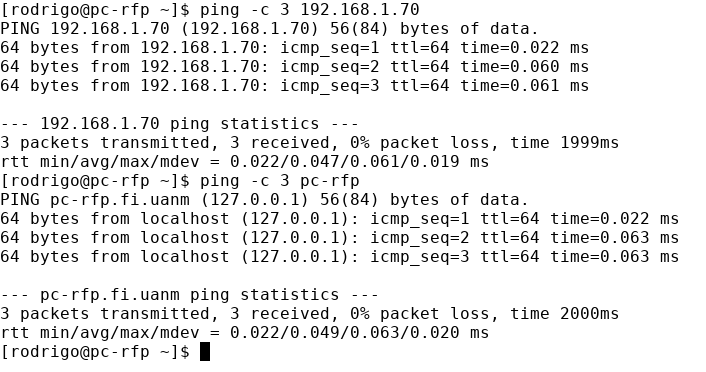
\includegraphics[width=10cm]{c01}    

\section*{C2. Explicación de las opciones -u -g -G}

De acuerdo al \textit{man page} de \texttt{useradd}:

\begin{itemize}
    \item \texttt{-u} o \texttt{--uid} $\langle$UID$\rangle$. Especifica el 
    valor númerico único del ID del usuario. No debe ser un valor negativo.
    \item \texttt{-g} o \texttt{--gid} $\langle$GROUP$\rangle$. Nos permite 
    definir el nombre de grupo o número para el grupo inicial (primario) del 
    usuario. El nombre de grupo especificado debe existir.
    \item \texttt{-G} o \texttt{--groups} $\langle$GROUP$\rangle$[,GROUP1,
    GROUP2,...]. Es una opción que nos permite indicar que el usuario pertenece 
    a los grupos listados en esta opción.
\end{itemize}

\section*{C3. Salida ejecución del validador}
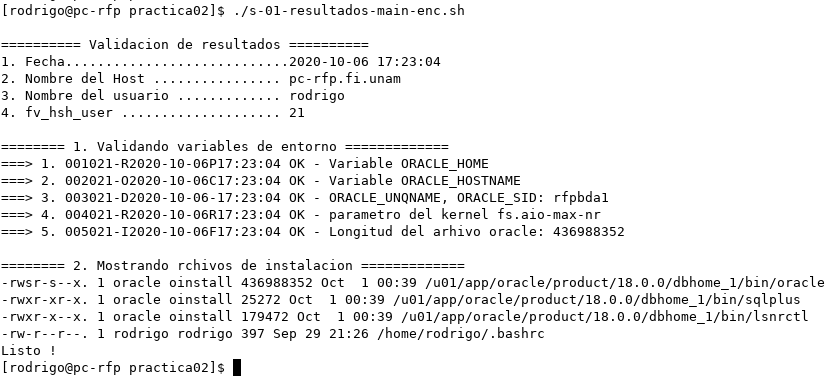
\includegraphics[width=16cm]{c03}    

\section*{Comentarios y conclusiones}

% Comentarios sobre la instalacion del software de bd
Realizar la instalación del \textit{software Oracle} en un distribución de Linux
soportada oficialmente por el manejador es muchísimo más sencillo que en uno que
no lo soporta (Distribuciones basadas en Debian o peor aún, en Arch Linux).
La instalación fue relativamente sencilla, solo tuvimos que ajustar algunos 
párametros del kernel y configurar los límites de algunos recursos del sistema.
Además por supuesto de agregar al usuario oracle con sus respectivos grupos.\\

Lo más importante que me llevo de esta práctica es que debo tener cuidado con 
las instancias que cree en un futuro, puesto que estoy cursando 
\textbf{Base de datos avanzadas} y \textbf{Base de datos distribuidas} al mismo
tiempo. El software se instala de la misma manera pero no puedo reutilizar 
las instancias.


\renewcommand\refname{Bibliografía}
\begin{thebibliography}{99}
    \bibitem{oracle} Oracle. \textit{Oracle Database Documentation} en 
        \texttt{https://docs.oracle.com/en/database/oracle/\\oracle-database/%
        index.html}
\end{thebibliography}

\end{document}
